%! TEX root = pedestrian.tex
% the main TeX file which is intended to compile, :VimtexReload after adjustment
   % this file should be included in the main file
% :h vimtex-tex-root
\documentclass[../rumukota.tex]{subfiles}
%ensure the class of docs

\begin{document}

\section{Pedestrian}%
\label{sec:Pedestarian}

\subsection{Definisi Pedestrian}%
\label{sub:definisi_pedestarian}

Pedestrian adalah para pejalan kaki, yang timbul karena adanya suatu kaitan kegiatan antara dua tempat atau yang jaraknya tidak begitu jauh. Umumnya mencapai jumlah yang cukup besar pada daerah perbelanjaan atau yang disering disebut sebagai Central Bussines District (CBD). Pedestrian berasal dari bahasa Yunani, yaitu dari kata *pedos* yang berarti kaki. Oleh karena itu, pedestrian dapat diartikan sebagai pejalan kaki atau orang yang berjalan kaki. Sementara itu, jalan merupakan media di atas permukaan bumi yang memudahkan manusia dalam melakukan pergerakan. Dengan demikian, pedestrian dalam konteks ini berarti pergerakan atau perpindahan manusia dari satu tempat sebagai titik awal ke tempat lain sebagai tujuan dengan menggunakan moda berjalan kaki. Secara harfiah, pedestrian juga diartikan sebagai *“person walking in the street”*, yaitu orang yang berjalan di jalan.

Fasilitas jalur pedestrian dibutuhkan pada:

\begin{enumerate}
	\item Daerah perkotaan yang memiliki jumlah penduduk tinggi.
	\item Jalan-jalan pasar dan kawasan perkotaan.
	\item Daerah dengan aktivitas kontinu yang tinggi, seperti kawasan pasar dan pusat kota.
	\item Lokasi dengan kebutuhan atau permintaan tinggi dalam periode singkat, seperti terminal bus, stasiun kereta api, sekolah, rumah sakit, dan lapangan olahraga.
	\item Lokasi dengan permintaan tinggi pada waktu tertentu, seperti lapangan atau gelanggang olahraga dan masjid.
	\item Daerah rekreasi (Iswanto, 2006).
\end{enumerate}

Pedestrian ways, atau yang biasa disebut trotoar, adalah jalur yang dirancang khusus untuk pejalan kaki. Jalur ini umumnya dibangun sejajar dengan jalan dan memiliki elevasi yang lebih tinggi dari permukaan jalan untuk menjamin keamanan pengguna. Jalur pedestrian tidak hanya berfungsi sebagai pelengkap ruang jalan, tetapi juga memiliki peran utama sebagai sarana bagi pejalan kaki untuk bergerak dan berpindah tempat dengan aman dan nyaman, tanpa rasa takut terhadap pengguna jalan lain maupun kendaraan (Setiawan, 2011).

Fungsi jalur pedestrian adalah untuk mengurangi gangguan bagi pejalan kaki saat berjalan di tempat umum serta mendorong aktivitas yang positif sehingga dapat mengurangi kerawanan kriminalitas. Jalur pedestrian juga berfungsi sebagai ruang gerak yang terpisah dari kendaraan bermotor. Jalur pedestrian yang ideal harus mampu mengakomodasi seluruh aktivitas pejalan kaki dengan lancar dan aman. Oleh karena itu, persyaratan ini perlu dipertimbangkan dalam perancangan jalur pejalan kaki.

Berikut adalah fungsi-fungsi jalur pedestrian:
\begin{enumerate}
	\item Pemisah jalur kendaraan dengan jalur pejalan kaki.
	\item Penghubung berbagai lokasi.
	\item Jalur fungsional menuju tempat lainnya.
	\item Menjadi tempat transit, termasuk halte, area istirahat, dan fasilitas lainnya.
	\item Wadah ruang gerak bagi pejalan kaki untuk melakukan berbagai aktivitas.
\end{enumerate}

Pada jalur pedestrian yang keberadaannya sangat diperlukan oleh pejalan kaki, umumnya terdapat elemen-elemen yang disebut sebagai perabot jalan (*street furniture*). Perabot jalan ini disesuaikan dengan fungsi kawasan dan digunakan pada area publik luar ruang. Fasilitas pelengkap ini harus memenuhi beberapa kriteria, yaitu bahan mudah diperoleh, mudah dirawat, tahan lama, aman, dan nyaman.

Berikut adalah beberapa elemen perabot jalan yang umumnya terdapat pada jalur pedestrian:
\begin{enumerate}
	\item Pohon atau tanaman peneduh, berfungsi sebagai tempat berteduh, penyejuk, pelindung, penyaring udara, serta memperindah jalur pedestrian.
	\item Patung, berfungsi untuk mempercantik jalur pedestrian dan menarik perhatian visual.
	\item Taman, berfungsi memperindah jalur pedestrian agar tidak terkesan gersang.
	\item Lampu, digunakan sebagai penerangan pada malam hari.
	\item Paving, yaitu material penutup permukaan seperti trotoar atau ubin yang rata.
	\item Tanda, berupa papan penunjuk arah dan informasi bagi pengguna jalan.
\end{enumerate}

Menurut Peraturan Menteri PUPR Nomor 03/PRT/M/2014 tentang Pedoman Penyediaan dan Pemanfaatan Prasarana dan Sarana Ruang Pejalan Kaki di Perkotaan, penempatan trotoar yang baik harus memenuhi beberapa syarat sebagai berikut:
\begin{enumerate}
	\item Trotoar dibangun di kawasan yang memiliki potensi pejalan kaki, seperti perumahan, pusat perbelanjaan, dan sekolah.
	\item Trotoar ditempatkan pada sisi luar bahu jalan. Apabila terdapat jalur parkir, maka trotoar ditempatkan di sisi luar jalur lalu lintas.
	\item Trotoar ditempatkan sedapat mungkin pada sisi dalam saluran drainase terbuka atau di atas saluran drainase yang tertutup.
\end{enumerate}

Faktor-faktor pendukung seperti kondisi fisik, ketersediaan area duduk, vegetasi atau pepohonan peneduh, pencahayaan, tanda arah, dan elemen lainnya sangat memengaruhi kenyamanan pejalan kaki. Jalur pejalan kaki yang fungsional mencakup dimensi fisik (panjang, lebar, dan ketinggian), aksesibilitas, karakteristik pengguna, frekuensi aktivitas, serta keterkaitan dengan lingkungan sekitarnya seperti kawasan permukiman, perkantoran, dan perdagangan.

Selain faktor fisik, terdapat pula faktor psikologis yang memengaruhi kualitas jalur pedestrian, yaitu keamanan dan kenyamanan. Keamanan berkaitan dengan sejauh mana jalur pejalan kaki mampu memberikan rasa aman, baik dari lalu lintas maupun dari lingkungan sekitarnya. Sementara itu, kenyamanan berkaitan dengan suasana, kelancaran sirkulasi, serta kelengkapan elemen pendukung yang memenuhi standar.

Ketidakberlanjutan jalur pedestrian dapat menimbulkan dampak negatif karena tidak memberikan ruang yang luas dan bebas bagi pengguna untuk beraktivitas. Jalur pedestrian yang baik adalah jalur yang memiliki rute berkesinambungan tanpa terputus, sehingga dapat digunakan kapan saja dan mampu mendukung berbagai aktivitas masyarakat.

Pembangunan jalur pedestrian tidak seharusnya hanya menjadi pelengkap ruang jalan, tetapi juga sebagai wadah utama bagi pejalan kaki untuk bergerak dan berpindah tempat dengan aman dan nyaman tanpa rasa takut terhadap pengguna lain atau kendaraan. Kurangnya rasa aman dan nyaman pada jalur pedestrian dapat menurunkan intensitas aktivitas masyarakat dan mengurangi kontribusi positif terhadap dinamika kawasan.

Jalur pejalan kaki merupakan ruang publik yang tidak hanya berfungsi secara fisik, tetapi juga dirasakan secara sosial oleh manusia. Di dalamnya terjadi interaksi sosial antar masyarakat, sehingga keberadaannya menjadi salah satu komponen penting dalam pembentukan kualitas ruang kota. Oleh karena itu, perancangan jalur pedestrian harus memperhatikan elemen-elemen desain kota agar fungsinya optimal sekaligus mampu memperkuat identitas kawasan.

Jalur pedestrian seharusnya diperuntukkan khusus bagi aktivitas pejalan kaki, bukan untuk penggunaan kendaraan, parkir, maupun kegiatan berdagang. Hal ini penting untuk menjaga keselamatan dan kenyamanan sirkulasi. Namun dalam praktiknya, jalur pejalan kaki sering kali tidak dirancang secara optimal, misalnya dipenuhi pedagang kaki lima atau memiliki perbedaan elevasi yang menyulitkan pergerakan. Oleh karena itu, diperlukan perencanaan yang lebih baik agar jalur pedestrian dapat berfungsi sesuai dengan tujuan utamanya, yaitu mendukung aktivitas pejalan kaki secara aman dan nyaman.

\subsection{Pengertian Kenyamanan Jalur Pedestrian}%
\label{sub:pengertian_kenyamanan_jalur_pedestrian}

Menurut Rustam Hakim dan Hardi Utomo, kenyamanan adalah segala hal yang menunjukkan penggunaan ruang secara tepat dan serasi, baik dengan karakteristik ruang itu sendiri maupun dengan berbagai unsur seperti bentuk, tekstur, warna, simbol, tanda, suara, kesan, intensitas pencahayaan, serta aroma dan unsur lainnya.

Fungsi jalan sangat berpengaruh terhadap proses aktivitas pergerakan manusia, sehingga sarana dan prasarana jalan harus direncanakan secara memadai dan tersistem untuk mendukung kelancaran aktivitas masyarakat umum. Unsur-unsur yang memengaruhi kenyamanan pada jalur pedestrian antara lain sebagai berikut:

\subsubsection{Sirkulasi}%
\label{ssub:sirkulasi}


Faktor sirkulasi memengaruhi tingkat kenyamanan dengan menyediakan pembagian ruang yang sesuai dengan tujuan penggunaannya, baik bagi pejalan kaki maupun kendaraan bermotor, serta melalui pengaturan sirkulasi antar ruang. Sirkulasi diartikan sebagai perputaran atau peredaran.

\tabitem Dimensi Jalur Pedestrian

Salah satu aspek penting dalam sirkulasi adalah dimensi jalur pedestrian. Perancangan dimensi prasarana jalur pejalan kaki harus memperhatikan standar minimum agar dapat mengakomodasi aktivitas pengguna secara optimal. Lebar minimum jalur pedestrian yang dibutuhkan umumnya disesuaikan dengan jenis penggunaan lahan di sekitarnya.

Lebar minimum jalur pedestrian berdasarkan penggunaan lahan dapat dilihat pada tabel berikut:



\begin{table}[h]
	\centering
	\begin{tabularx}{\textwidth}{p{20mm}lX}
		\hline
		No.  &  Penggunaan Lahan Sekitarnya     &  Lebar Minimum (m)  \\ \hline
		1    &  Perumahan                       &  1,6  \\
		2    &  Perkantoran                     &  2  \\
		3    &  Industri                        &  2  \\
		4    &  Sekolah                         &  2  \\
		5    &  Terminal/Stop Bus/TPKPU         &  2  \\
		6    &  Pertokoan/Perbelanjaan/Hiburan  &  2  \\
		7    &  Jembatan/Terowongan             &  1  \\
	\end{tabularx}
	\caption{Lebar Minimum Pedestrian Menurut Penggunaan Lahan Sekitarnya}
\end{table}


\tabitem Waktu dan Volume Pejalan Kaki

Menurut Peraturan Menteri Pekerjaan Umum No: 03/PRT/M/2014, tingkat pelayanan pejalan kaki dibagi menjadi 6 standar, antara lain :

\begin{itemize}

	\item Standar A
	\item[] Standar A, para pejalan kaki dapat berjalan menggunakan bebas, termasuk dapat memilih arah berjalan dengan bebas, menggunakan kecepatan yang relatif cepat tanpa menimbulkan gangguan antar pejalan kaki. Luas jalur pejalan kaki
	      ≥ 12 m2 per orang dengan arus pejalan kaki < 16 orang per menit per meter.
	\item Standar B
	\item[] Standar B, para pejalan kaki masih dapat berjalan dengan nyaman dan cepat tanpa mengganggu pejalan kaki lainnya, namun keberadaan pejalan kaki yang lainnya sudah mulai berpengaruh pada arus pejalan kaki. Luas jalur pejalan kaki ≥ 3,6 m2 per orang dengan arus pejalan kaki >16-23 orang per menit per meter.

	\item Standar C
	      Standar C, para pejalan kaki dapat bergerak dengan arus yang searah secara normal walaupun pada arah yang berlawanan akan terjadi persinggungan kecil, dan relative lambat karena keterbatasan ruang antar pejalan kaki. Luas jalur pejalan kaki ≥ 2,2-3,5 m2/orang dengan arus pejalan kaki >23-33 orang per menit per meter.

	\item Standar D
	\item[] Standar D, para pejalan kaki dapat berjalan dengan arus normal, namun harus sering berganti posisi dan merubah kecepatan karena arus berlawanan pejalan kaki memiliki potensi untuk dapat menimbulkan konflik. Standar ini masih menghasilkan arus ambang nyaman untuk pejalan kaki tetapi berpotensi timbulnya persinggungan dan interaksi antar pejalan kaki. Luas jalur pejalan kaki ≥ 1,2–2,1 m2/orang dengan arus pejalan kaki >33-49 orang per menit per meter.

	\item Standar E
	\item[] Standar E, para pejalan kaki dapat berjalan dengan kecepatan yang sama, namun pergerakan akan relatif lambat dan tidak teratur ketika banyaknya pejalan kaki yang berbalik arah atau berhenti. Standar E mulai tidak nyaman untuk dilalui tetapi masih merupakan ambang bawah dari kapasitas rencana ruang pejalan kaki. Luas jalur pejalan kaki ≥ 0,5–1,3 m2/orang dengan arus pejalan kaki >49- 75 orang per menit per meter.

	\item Standar F
	\item[] Standar F, para pejalan kaki berjalan dengan kecepatan arus yang sangat lambat dan terbatas karena sering terjadi konflik dengan pejalan kaki yang searah atau berlawanan. Standar F sudah tidak nyaman dan sudah tidak sesuai dengan kapasitas ruang pejalan kaki. Luas jalur pejalan kaki < 0,5 m2/orang dengan arus pejalan kaki beragam.

\end{itemize}

\subsubsection{Bentuk}%
\label{ssub:bentuk}

Bentuk elemen harus diubah sesuai dengan ukuran standar manusia sehingga bentuk skala memiliki rasa nyaman. Misalnya, tingkat permukaan lantai pedestrian dan jalur kendaraan, pembatas jalur pejalan kaki, pelandaian yang tepat dan tidak terlalu curam, tempat duduk, dan lain sebagainya. Kemiringan atau pelandaian diletakkan di pintu masuk, tempat penyebrangan, dan persimpangan pejalan kaki.

\tabitem Ketinggian Pedestrian

Jalur pejalan kaki adalah ruang yang digunakan untuk berjalan kaki atau berkursi roda bagi penyandang disabilitas secara mandiri dan dirancang berdasarkan kebutuhan orang untuk bergerak aman, mudah, nyaman dan tanpa hambatan. Jalur pejalan kaki setidaknya memiliki lebar 1,8 - 3,0 meter atau lebih. Hal ini bertujuan untuk memenuhi tingkat pelayanan yang diinginkan khususnya pada kawasan yang memiliki intensitas pejalan kaki yang tinggi. Untuk lebar minimum pada kawasan tertentu dapat diuraikan sebagai berikut:

\begin{itemize}
	\item Kawasan pertokoan dan perdagangan adalah sebesar 2 meter.
	\item Kawasan jalan lokal dan jalan kolektor adalah sebesar 1,2 meter.
	\item Kawasan jalan arteri adalah sebesar 1,8 meter.
\end{itemize}

Jalur pejalan kaki tidak boleh memiliki lebar kurang dari 1,2 meter yang merupakan lebar minimum. Perbedaan tinggi maksimal antara jalur pejalan kaki dengan jalur kendaraan adalah sebesar 0,2 meter (20 centimeter) (Perencanaan Teknis Fasilitas Pejalan Kaki, 2018)

\tabitem Pelandaian

Fungsi pelandaian adalah :

\begin{enumerate}
	\item Untuk memfasilitasi perubahan tinggi secara baik
	\item Untuk memfasilitasi pejalan kaki yang menggunakan kursi roda
\end{enumerate}
Persyaratan khusus untuk pelandaian adalah sebagai berikut :

\begin{enumerate}
	\item Tingkat kelandaian maksimum 12 \% ( 1:8) dan disarankan 8\% (1:12). Untuk mencapai nilai tersebut, pelandaian sedapat mungin berada dalam zona jalur fasilitas. Bila perlu, ketinggian Pedestrian bisa diturunkan.
	\item Area landau harus memiliki penerangan yang cukup. Contoh pelandaian pada tempat penyebrangan pejalan kaki.
\end{enumerate}

\begin{figure}
	\begin{center}
		
\includegraphics[width=.82\textwidth]{pelandaian}
		% filename may not contain space but _
	\end{center}
	\caption{Pelandaian di Tempat Penyebrangan Pejalan Kaki}
	\label{fig:pelandaian}
\end{figure}

Cara pengaturan jalan masuk dapat dilakukan dengan menggunakan pelandaian kerb tegak lurus, pelandaian kerb kombinasi, dan pelandaian kerb paralel.

Tujuan dilakukannya pengaturan jalan masuk:

a)	Mengaruangi konflik antara pejalan kaki dan kendaraan
b)	Menyediakan akses bagi pejalan kaki
c)	Meningkatkan visibilitas antara mobil dan pejalan kaki di jalan masuk.


\begin{figure}
	\begin{center}
		
\includegraphics[width=.82\textwidth]{pelandaian_kerb}
		% filename may not contain space but _
	\end{center}
	\caption{Jalan Masuk dan Pelandaian Kerb Yang Tegak Lurus}
	\label{fig:kerb}
\end{figure}

\begin{figure}
	\begin{center}
		
\includegraphics[width=.82\textwidth]{kerb_2}
		% filename may not contain space but _
	\end{center}
	\caption{Jalan Masuk dan Pelandaian Kerb Kombinasi}
	\label{fig:kerb_kombinasi}
\end{figure}

\begin{figure}
	\begin{center}
		
\includegraphics[width=.82\textwidth]{kerb_3}
		% filename may not contain space but _
	\end{center}
	\caption{Jalan Masuk dan Pelandaian Kerb Kombinasi Paralel}
	\label{fig:kerb_paralel}
\end{figure}

\tabitem Bangku atau Stop Point

Bangku atau titik berhenti dalam desain perkotaan berfokus pada fungsi, lokasi, dan desain bangku untuk mendukung kenyamanan, keselamatan, dan interaksi sosial.A

\begin{description}
	\item[Fungsi:] Bangku menyediakan tempat istirahat, pertemuan, dan sosialisasi di ruang publik. Mereka memberikan kesempatan bagi pejalan kaki untuk berhenti sejenak dan menikmati lingkungan sekitar.
	\item[Lokasi:] Bangku sebaiknya ditempatkan di area dengan aktivitas pejalan kaki yang tinggi seperti koridor perbelanjaan, halte transportasi, dan taman. Lokasi ideal adalah setiap 50-100 meter di area dengan aktivitas intens, untuk memastikan akses yang mudah bagi semua, termasuk penyandang disabilitas.
	\item[Desain:] Desain bangku harus mempertimbangkan kenyamanan dan keamanan. Bangku yang baik memiliki bahan yang tahan cuaca, mudah dipelihara, dan dapat mengakomodasi berbagai kebutuhan pengguna. Mereka juga harus ditempatkan dengan cara yang mendukung interaksi sosial, misalnya dengan menyusun bangku pada sudut tertentu untuk memfasilitasi percakapan kelompok(Ozyavuz, 2013).
\end{description}


\subsubsection{Keamanan}%
\label{ssub:keamanan}
Keamanan adalah kondisi yang diinginkan oleh pejalan kaki tanpa mengorbankan kenyamanan mereka. Keamanan tidak hanya berkaitan dengan aspek kriminalitas, tetapi juga dengan faktor-faktor seperti pencahayaan yang memadai, keberadaan pagar pembatas, serta kondisi jalur pejalan kaki yang tidak licin dan tidak berlubang. Lampu penerangan fasilitas pejalan kaki Lampu penerangan fasilitas pejalan kaki adalah untuk memberikan pencahayaan pada malam hari agar area fasilitas pejalan kaki dapat lebih aman dan nyaman Lampu penerangan diletakkan pada jalur fasilitas.


\tabitem Penerangan Jalan

Lampu penerangan jalan adalah lampu yang digunakan untuk penerangan jalan dimalam hari sehingga mempermudah pejalan kaki, pesepeda dan pengendara kendaraan dapat melihat dengan lebih jelas atau medan yang akan dilalui pada malam hari, sehingga dapat meningkatkan keselamatan lalu lintas, kenyamanan pengguna jalan dan memberikan keamanan dari aksi kriminalitas.
Lampu penerangan jalan yang baik adalah suatu unit lengkap yang terdiri dari sumber cahaya (lampu), elemen-elemen optik (pemantul), penyebar, elemenelemen elektrik, struktur penopang yang terdiri dari lengan penopang vertikal dan pondasi tiang lampu. Dimana penerangan jalan umum biasa dipasang pada bagian kanan dan kiri jalan atau di tengah (median jalan) yang digunakan untuk menerangi jalan maupun lingkungan di sekitar jalan yang diperlukan. Terletak setiap 10 meter dengan tinggi maksimal 4 meter, dan bahan yang digunakan adalah bahan dengan daya tahan yang tinggi seperti metal \& beton cetak(Yogha Goetama, 2017).

\tabitem Jalur Pejalan Kaki bagi Penyandang Tuna Netra

\begin{figure}
	\begin{center}
		
\includegraphics[width=.82\textwidth]{ruang_gerak}
		% filename may not contain space but _
	\end{center}
	\caption{Ruang Gerak bagi Tuna Netra}
	\label{fig:tuna_netra}
\end{figure}
Bagi pejalan kaki yang berkebutuhan khusus (tuna netra dan yang terganggu penglihatan), membutuhkan informasi khusus pada permukaan lajur pejalan kaki. Informasi tersebut disebut lajur pemandu. Lajur pemandu terdiri dari:


\begin{itemize}

	\item Ubin/blok kubah sebagai peringatan, dengan tipe seperti Gambar berikut
	\item[] \begin{figure}
		      \begin{center}
			      
\includegraphics[width=.82\textwidth]{blok_peringatan}
			      % filename may not contain space but _
		      \end{center}
		      \caption{Blok Peringatan}
		      \label{fig:blok_peringatan}
	      \end{figure}

	\item Ubin/blok garis sebagai pengarah, dengan tipe seperti Gambar berikut:

	\item[] \begin{figure}
		      \begin{center}
			      
\includegraphics[width=.82\textwidth]{blok_arah}
			      % filename may not contain space but _
		      \end{center}
		      \caption{Blok Pengarah}
		      \label{fig:blok_pengarah}
	      \end{figure}

\end{itemize}

\tabitem Jalur Pejalan Kaki bagi Pengguna Kursi Roda

\begin{figure}
	\begin{center}
		
\includegraphics[width=.82\textwidth]{ruang_kursi_roda}
		% filename may not contain space but _
	\end{center}
	\caption{Ruang Gerak bagi Pengguna Kursi Roda}
	\label{fig:kursi_roda}
\end{figure}

\tabitem Jembatan Penyeberangan Jalan

Penataan khusus pembangunan jalur pejalan kaki yang mengikuti pedoman No. 027/T/Bt/1995 tentang Tata Cara Perencanaan Jembatan Penyeberangan Untuk Pejalan Kaki di Kawasan Perkotaan. Jembatan penyeberangan untuk pejalan kaki adalah bangunan jembatan yang diharapkan atau dirancang untuk menyeberang pejalan kaki dari satu sisi jalan ke sisi jalan yang berlawanan. Jembatan peyeberangan pejalan kaki harus dibangun dengan kontruksi yang cukup kuat dan mudah untuk dipelihara. Jembatan penyeberangan orang memiliki lebar minimum 2 (dua) meter dan kemiringan atau kelandaain maksimal 20º. Dengan asumsi bahwa jika jembatan penyeberangan juga digunakan bagi sepeda maka lebar minimum 2,75 m.

Ketentuan teknis konstruksi jembatan penyeberangan mengikuti No. 027/T/Bt/1995 tentang Tata cara perencanaan jembatan penyeberangan untuk pejalan kaki di kawasan perkotaan. Jembatan penyeberangan pejalan kaki merupakan bangunan jembatan yang diperuntukkan untuk menyeberang pejalan kaki dari satu sisi jalan ke sisi jalan yang lainnya. Jembatan penyeberang pejalan kaki harus dibangun dengan konstruksi yang kuat dan mudah dipelihara. Jembatan penyeberangan pejalan kaki memiliki lebar minimum 2 (dua) meter dan kelandaian tangga maksimum 20º.Bila jembatan penyeberangan juga diperuntukkan bagi sepeda, maka lebar minimal adalah 2,75 m.

Jembatan penyeberangan pejalan kaki harus dilengkapi dengan pagar yang memadai. Di bagian tengan tangga peyeberangan harus ada harus dilengkapi dengan pelandaian yang bisa dimanfaatkan sebagai fasilitas untuk pengguna kursi roda dan bagi penyandang disabilitas. Area dan pengembangan jembatan pejalan kaki harus sesuai dengan kebutuhan dan kebutuhan orang yang berjalan kaki. Penempatan jembatan penyeberangan tidak boleh mengurangi lebar jalan.

\begin{figure}
	\begin{center}
		
\includegraphics[width=.82\textwidth]{jembatan}
		% filename may not contain space but _
	\end{center}
	\caption{Perspektif Jembatan Penyebrangan Orang}
	\label{fig:jembatan_orang}
\end{figure}

Beberapa tipikal jembatan penyeberangan:
\begin{figure}
	\begin{center}
		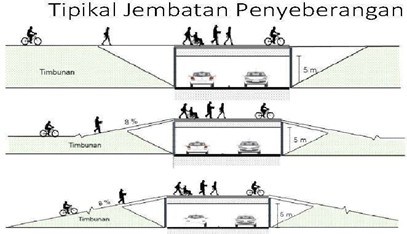
\includegraphics[width=.82\textwidth]{../figures/tipikal_jembatan.jpg}
		% filename may not contain space but _
	\end{center}
	\caption{Tipikal Jembatan penyebrangan}
	\label{fig:tipikal_jembatan}
\end{figure}

\tabitem Halte

Keberadaan pemberhentian sementara atau halte tidak boleh mengurangi lebar efektif trotoar. Halte dapat ditempatkan di depan ataupun belakang lajur pejalan kaki. Halte juga harus dilengkapi dengan akses pejalan kaki berkebutuhan khusus, dan fasilitas pendukung seperti tempat duduk, atap peneduh, dan kelengkapan lainnya.

\begin{figure}
	\begin{center}
		
\includegraphics[width=.82\textwidth]{halte}
		% filename may not contain space but _
	\end{center}
	\caption{Posisi Halte di Belakang Pedestrian}
	\label{fig:halte}
\end{figure}

Jarak yang umumnya digunakan penentuan jarak antara halte dan/atau tempat pemberhentian bis adalah 300 m.

\begin{figure}
	\begin{center}
		
\includegraphics[width=.82\textwidth]{halte_khusus}
		% filename may not contain space but _
	\end{center}
	\caption{Akses Pejalan Kaki disabilitas di Halte}
	\label{fig:}
\end{figure}


\subsubsection{Rambu Lalu Lintas}%
\label{ssub:rambu_lalu_lintas}


Penempatan rambu dan marka jalan harus diperhitungkan secara efisien untuk memastikan keselamatan lalu lintas. Marka jalan dimaksudkan sebagai piranti pengingat kepada pengemudi untuk berhati-hati dan bila diperlukan berhenti pada lokasi yang tepat untuk memberikan kesempatan kepada pejalan kaki menggunakan fasilitas dengan selamat. Pengaturan dengan marka jalan harus diupayakan untuk mampu memberikan perlindungan pada pengguna jalan yang lebih lemah, seperti pada pejalan kaki.
Rambu diletakan pada jalur fasilitas, pada titik interaksi sosial, pada jalur dengan arus orang padat, dengan besaran sesuai kebutuhan, dan bahan yang digunakan terbuat dari bahan yang memiliki daya tahan yang tinggi, dan tidak menimbulkan efek silau.


\subsubsection{Kebersihan}%
\label{ssub:kebersihan}

Kebersihan adalah kondisi yang diharapkan untuk menciptakan suasana yang positif dan menarik di lokasi tersebut. Ini mencakup pemeliharaan jalur pejalan kaki agar bebas dari tumpukan sampah dan bau tidak sedap, serta memperhatikan jenis tumbuhan yang dapat menyebabkan tumpukan sampah organik seperti daun dan buah. Kebersihan biasanya dikaitkan dengan pengelolaan sampah dan penataan drainase. Sehingga tong atau tempat sampah harus diletakkan pada tempat yang nyaman tentunya. Tempat sampah diletakkan setiap 20 meter dengan ukuran tergantung pada situasi, dan bahan yang digunakan adalah bahan dengan ketangguhan tinggi seperti logam dan beton cor.

\tabitem Penyediaan Tempat Sampah
Tempat sampah diletakan pada jalur fasilitas. Penempatan tempat sampah pada fasilitas pejalan kaki hanya untuk menampung sampah yang dihasilkan oleh pejalan kaki dan bukan untuk menampung sampah rumah tangga di sekitar fasilitas pejalan kaki. Tempat sampah terletak setiap 20 meter serta pada titik-titik pertemuan (misalnya persimpangan), dengan besaran sesuai kebutuhan, dan bahan yang digunakan adalah bahan dengan daya tahan yang tinggi seperti metal dan beton cetak.A

\tabitem Penataan Drainase

Drainase terletak berdampingan atau di bawah dari fasilitas pejalan kaki. Drainase berfungsi sebagai penampung dan jalur aliran air pada fasilitas pejalan kaki. Keberadaan drainase akan dapat mencegah terjadinya banjir dan genangan- genangan air pada saat hujan. Dimensi minimal drainase adalah lebar 50 cm dan tinggi 50 cm.

\subsubsection{Keindahan}%
\label{ssub:keindahan}

\tabitem Elemen Perkerasan

Penggunaan elemen material pada trotoar merupakan suatu hal yang penting untuk kenyamanan dan keamanan pejalan kaki. Pemenuhan elemen-elemen material yang digunakan dalam pedestrian bukan tanpa alasan. Pemilihan material mempertimbangkan kegunaan, estetika, dan biaya. Menurut Harksoso, dkk (2013) elemen-elemen material perkerasan yang digunakan pada jalur pedestrian adalah paving (beton), batu, atau bata.
\tabitem Komposisi Penyusunan Vegetasi

Keindahan merupakan hal yang perlu diperhatikan sekali dalam hal penciptaan kenyamanan karena hal tersebut dapat mencakup masalah kepuasan batin dan kepuasan mata. Demikian juga pada eksistensi keindahan di suatu jalur jalan raya termasuk trotoar, harus selalu terhindar dari ketidak beraturan bentuk, warna, atau pola aktivitas manusia yang ada di dalamnya. Pemandangan sebagian besar didasarkan pada estetika (buatan manusia) tetapi pada beberapa hal juga berhubungan dengan konservasi dan preservasi. Untuk memperoleh kenyamanan yang optimal, maka perlu memperhatikan beberapa segi seperti komposisi penyusunan tanaman atau vegetasi dan elemen pengkerasan. Konsep penataan jarak tanaman pohon pada jalur pedestrian 15-20 meter agar vegetasi tidak menghalangi pandangan kebangunan.

\begin{figure}
	\begin{center}
		
\includegraphics[width=.82\textwidth]{fasilitas_pohon}
		% filename may not contain space but _
	\end{center}
	\caption{Fasilitas Pohon Peneduh atau Vegetasi}
	\label{fig:vegetasi_pohon}
\end{figure}

\subsection{Pengaruh PKL}%
\label{sub:pengaruh_pkl}
Pengaruh dapat didefinisikan sebagai kekuatan atau efek yang dimiliki oleh suatu entitas atau individu terhadap pihak lain, yang dapat mengubah pemikiran, perasaan, atau tindakan. Pengaruh merupakan hubungan sebab-akibat antara pihak yang memengaruhi dan pihak yang terpengaruh. Pengaruh dapat muncul dalam berbagai konteks sosial, psikologis, dan komunikasi.

Pengaruh juga dapat diartikan sebagai nilai kualitas suatu media dalam menyampaikan pesan. Selain itu, pengaruh merupakan kemampuan individu atau kelompok dalam masyarakat yang memiliki sifat kosmopolitan, inovatif, kompeten, serta mudah dijangkau, baik secara formal maupun informal, untuk memengaruhi pihak lain. Pengaruh juga merupakan kapabilitas untuk memodifikasi tindakan, perspektif, atau perilaku individu lain melalui berbagai metode seperti keterlibatan, kepemimpinan, serta pendekatan lainnya. Di sisi lain, pengaruh dapat dipahami sebagai kapasitas seseorang atau suatu situasi dalam memodifikasi perilaku atau keyakinan individu.

Keberadaan pedagang kaki lima (PKL) memberikan pengaruh yang tidak dapat dihindari karena bersinggungan langsung dengan kondisi jalur pedestrian. Dampak dari keberadaan PKL dapat dibagi menjadi dua, yaitu dampak positif dan dampak negatif.

Dampak positif dari keberadaan PKL antara lain terpenuhinya kebutuhan barang harian dengan harga yang terjangkau serta modal usaha yang relatif kecil karena tidak memerlukan biaya sewa tempat.

Sementara itu, dampak negatifnya adalah pemanfaatan ruang terbuka publik sebagai area berdagang karena memiliki potensi besar untuk menarik konsumen. Hal ini menyebabkan pejalan kaki harus berbagi ruang atau bahkan berdesakan dengan aktivitas PKL. Selain itu, kepadatan pada jalur pedestrian juga dapat menimbulkan gangguan keamanan, seperti tindak kriminal.


\subsection{Pengertian Pejalan Kaki}%
\label{sub:pengertian_pejalan_kaki}

Pejalan kaki adalah istilah dalam transportasi yang merujuk pada individu yang berjalan di jalur pejalan kaki, termasuk trotoar dan lintasan khusus. Untuk menjamin keselamatan, pejalan kaki diharapkan menggunakan fasilitas penyeberangan yang telah disediakan. Namun, dalam praktiknya sering terjadi konflik antara pejalan kaki dan kendaraan bermotor, karena keberadaan pejalan kaki kerap terabaikan. Oleh karena itu, penting untuk menyediakan fasilitas yang memadai serta perawatan yang baik bagi pejalan kaki tanpa memposisikan mereka sebagai pengguna jalan kelas dua dibandingkan pemilik kendaraan.

Menurut peraturan lalu lintas dan angkutan jalan, pejalan kaki adalah setiap orang yang berjalan di ruang lalu lintas jalan. Karena aktivitasnya yang bergerak, pejalan kaki merupakan bagian dari sistem pergerakan lalu lintas. Oleh sebab itu, pejalan kaki memiliki hak dan kewajiban dalam berlalu lintas serta berhak memperoleh fasilitas pendukung guna menjamin keselamatan.

Secara umum, pejalan kaki juga dapat diartikan sebagai orang yang berjalan di lintasan pejalan kaki, baik di pinggir jalan, trotoar, lintasan khusus, maupun saat menyeberang jalan. Dalam rangka menjaga keselamatan, pejalan kaki seharusnya berjalan pada bagian jalan yang diperuntukkan bagi mereka dan menyeberang pada tempat penyeberangan yang telah disediakan.

\subsection{Pengertian Pedagang Kaki Lima}%
\label{sub:pengertian_pedagang_kaki_lima}

Pedagang kaki lima (PKL) merupakan salah satu bentuk kegiatan dalam sektor informal. Istilah ini pertama kali diperkenalkan pada masa pemerintahan Raffles untuk merujuk pada area berukuran lima kaki yang digunakan sebagai jalur pejalan kaki di tepi jalan. Area tersebut kemudian dimanfaatkan sebagai tempat berjualan oleh pedagang kecil, sehingga para pedagang yang menggunakan area tersebut dikenal sebagai pedagang jalanan.

PKL dapat dikelompokkan ke dalam beberapa kategori berdasarkan jenis komoditas yang ditawarkan, seperti makanan mentah, makanan siap saji, barang dagangan, dan jasa. Keberadaan PKL tidak terlepas dari ketidakseimbangan antara jumlah tenaga kerja dan peluang kerja yang tersedia. Kondisi ini mendorong sebagian masyarakat untuk mencari alternatif mata pencaharian di sektor informal, salah satunya dengan menjadi pedagang jalanan.

Pedagang kaki lima umumnya muncul akibat terbatasnya peluang kerja di sektor formal, sehingga masyarakat beralih ke sektor informal untuk memenuhi kebutuhan hidup. Oleh karena itu, lokasi keberadaan PKL sering kali berada pada area yang sebenarnya tidak diperuntukkan bagi kegiatan perdagangan.

Pada masa pemerintahan Raffles, diberlakukan aturan yang mengharuskan pedagang informal menjaga jarak sekitar lima kaki dari bangunan formal di pusat kota. Tujuan dari aturan ini adalah untuk menciptakan kenyamanan, khususnya bagi pejalan kaki, sekaligus tetap memberikan ruang bagi pedagang informal untuk berjualan. Seiring waktu, istilah pedagang kaki lima menjadi dikenal luas oleh masyarakat.

Dalam bidang perdagangan, PKL termasuk dalam sektor informal yang bersifat sederhana dan sering kali tidak memiliki legalitas formal. Berdasarkan kondisi operasionalnya, PKL dapat dibedakan menjadi dua kategori sebagai berikut:
\begin{enumerate}
	\item PKL Tertata

	      PKL tertata adalah pedagang kaki lima yang menjalankan usahanya di lokasi yang telah ditentukan atau diizinkan oleh pemerintah daerah. Pedagang dalam kategori ini umumnya memiliki izin resmi dan diwajibkan untuk mematuhi berbagai ketentuan, seperti membayar retribusi serta menjaga kebersihan, keindahan, dan keamanan lingkungan.

	\item PKL Binaan

	      PKL binaan adalah pedagang kaki lima yang beroperasi di lokasi yang tidak diizinkan oleh pemerintah daerah. Meskipun tidak memiliki izin resmi dan tidak dikenakan retribusi, keberadaan mereka tetap diawasi dan dibina oleh pemerintah agar dapat berkembang menjadi pedagang yang tertib.
\end{enumerate}

Seiring dengan bertambahnya jumlah PKL, kebutuhan akan penyediaan ruang yang memadai menjadi semakin penting. Di sisi lain, keberadaan PKL sering dianggap mengganggu ketertiban dan kebersihan kota. Pertumbuhan PKL yang pesat juga dapat menyebabkan ruang kota terasa semakin sempit dan kurang nyaman.

Dalam menghadapi kondisi tersebut, pemerintah kota sering mengambil kebijakan relokasi PKL sebagai upaya penataan. Namun, kebijakan ini kerap menimbulkan penolakan dari para pedagang karena dianggap merugikan dan tidak memberikan solusi yang adil. Selain itu, permasalahan seperti belum tersedianya lokasi yang layak dan kurangnya kepastian dari pemerintah menjadi tantangan tersendiri bagi para PKL. Oleh karena itu, harapan akan tersedianya fasilitas dan lahan khusus yang memadai bagi PKL menjadi hal yang sangat penting untuk mewujudkan lingkungan kota yang tertib, bersih, dan nyaman.










\bibliographystyle{apalike}
\bibliography{../filename.bib} % required for citecompletion, not work in mainfile
\end{document}

